\documentclass[letterpaper,10pt]{article}

\usepackage{enumitem}
\usepackage{titling}
\usepackage{listings,listings-rust}
\usepackage{url}
\usepackage{soul}
\usepackage{hyperref}
\usepackage{setspace}
\usepackage{subfig}
\usepackage{sectsty}
\usepackage{pdfpages}
\usepackage{colortbl}
\usepackage{multirow}
\usepackage{multicol}
\usepackage{relsize}
\usepackage{amsmath}
\usepackage{wasysym}
\usepackage{fancyvrb}
\usepackage[yyyymmdd]{datetime}
\usepackage{amsmath,amssymb,amsthm,graphicx,xspace}
\usepackage[titlenotnumbered,noend,noline]{algorithm2e}
\usepackage[compact]{titlesec}
\usepackage{XCharter}
\usepackage[T1]{fontenc}
\usepackage[scaled]{beramono}
\usepackage[normalem]{ulem}
\usepackage{booktabs}
\usepackage{tikz}
\usetikzlibrary{arrows.meta,automata,shapes,trees,matrix,chains,scopes,positioning,calc,decorations.pathreplacing}
\tikzstyle{block} = [rectangle, draw, fill=blue!20, 
    text width=2.5em, text centered, rounded corners, minimum height=2em]
\tikzstyle{bw} = [rectangle, draw, fill=blue!20, 
    text width=4em, text centered, rounded corners, minimum height=2em]

\definecolor{namerow}{cmyk}{.40,.40,.40,.40}
\definecolor{namecol}{cmyk}{.40,.40,.40,.40}
\renewcommand{\dateseparator}{-}

\let\LaTeXtitle\title
\renewcommand{\title}[1]{\LaTeXtitle{\textsf{#1}}}

\lstset{basicstyle=\footnotesize\ttfamily,breaklines=true}

\newcommand{\CPP}{C\nolinebreak\hspace{-.05em}\raisebox{.4ex}{\tiny\bf +}\nolinebreak\hspace{-.10em}\raisebox{.4ex}{\tiny\bf +}}
\def\CPP{{C\nolinebreak[4]\hspace{-.05em}\raisebox{.4ex}{\tiny\bf ++}}}

\newcommand{\handout}[5]{
  \noindent
  \begin{center}
  \framebox{
    \vbox{
      \hbox to 5.78in { {\bf ECE459: Programming for Performance } \hfill #2 }
      \vspace{4mm}
      \hbox to 5.78in { {\Large \hfill #4  \hfill} }
      \vspace{2mm}
      \hbox to 5.78in { {\em #3 \hfill \today} }
    }
  }
  \end{center}
  \vspace*{4mm}
}

\newcommand{\lecture}[3]{\handout{#1}{#2}{#3}{Lecture#1}}
\newcommand{\tuple}[1]{\ensuremath{\left\langle #1 \right\rangle}\xspace}

\addtolength{\oddsidemargin}{-1.000in}
\addtolength{\evensidemargin}{-0.500in}
\addtolength{\textwidth}{2.0in}
\addtolength{\topmargin}{-1.000in}
\addtolength{\textheight}{1.75in}
\addtolength{\parskip}{\baselineskip}
\setlength{\parindent}{0in}
\renewcommand{\baselinestretch}{1.5}
\newcommand{\term}{Winter 2020}

\singlespace


\begin{document}

\lecture{ 3 --- Rust: Borrowing, Slices, Concurrency }{\term}{Jeff Zarnett}

\section*{Borrowing and References}
We've already seen that ownership is a concept in Rust that can come with a couple of unintended consequences, like accidentally giving an argument to a function that we still need later. Rust allows us the idea of ``borrowing'' -- you need to use the data for something but you also promise you'll give it back. It allows data to be shared, but the sharing has to be done in a controlled and safe way to prevent the possibility of race conditions.

Rust's compiler analyzes all the borrowing that takes place in the program using the \textit{borrow checker}. If the borrow checker is not certain that your code is perfectly safe, it will say no (and produce a compile time error). This can be a little bit frustrating, because the analysis is not perfect and errs on the side of caution. Eventually we will introduce some ways that you can tell the borrow checker that you guarantee the code is safe, but you have to be sure, otherwise all the usual bad things can happen!

The feature that we need for the concept of borrowing is the \textit{reference}. To indicate that you want to use a reference, use the \texttt{\&} operator. The reference operator is appears both on the function definition and the invocation, to make sure there's no possibility of confusion as to whether a reference is being expected/provided or ownership is to be transferred.  Consider this example from the official docs~\cite{rustdocs}:

\begin{lstlisting}[language=Rust]
fn main() {
    let s1 = String::from("hello");
    let len = calculate_length(&s1);
    println!("The length of '{}' is {}.", s1, len);
}

fn calculate_length(s: &String) -> usize {
    s.len()
}
\end{lstlisting}

So when we invoke the \texttt{calculate\_length} function, ownership of the string is not transferred, but instead a reference to it is provided. The reference goes out of scope at the end of the function where it was used, removing it from consideration. A reference is not the same as ownership and the reference cannot exist without the original owner continuing to exist. That is represented in the official docs by this diagram:

\begin{center}
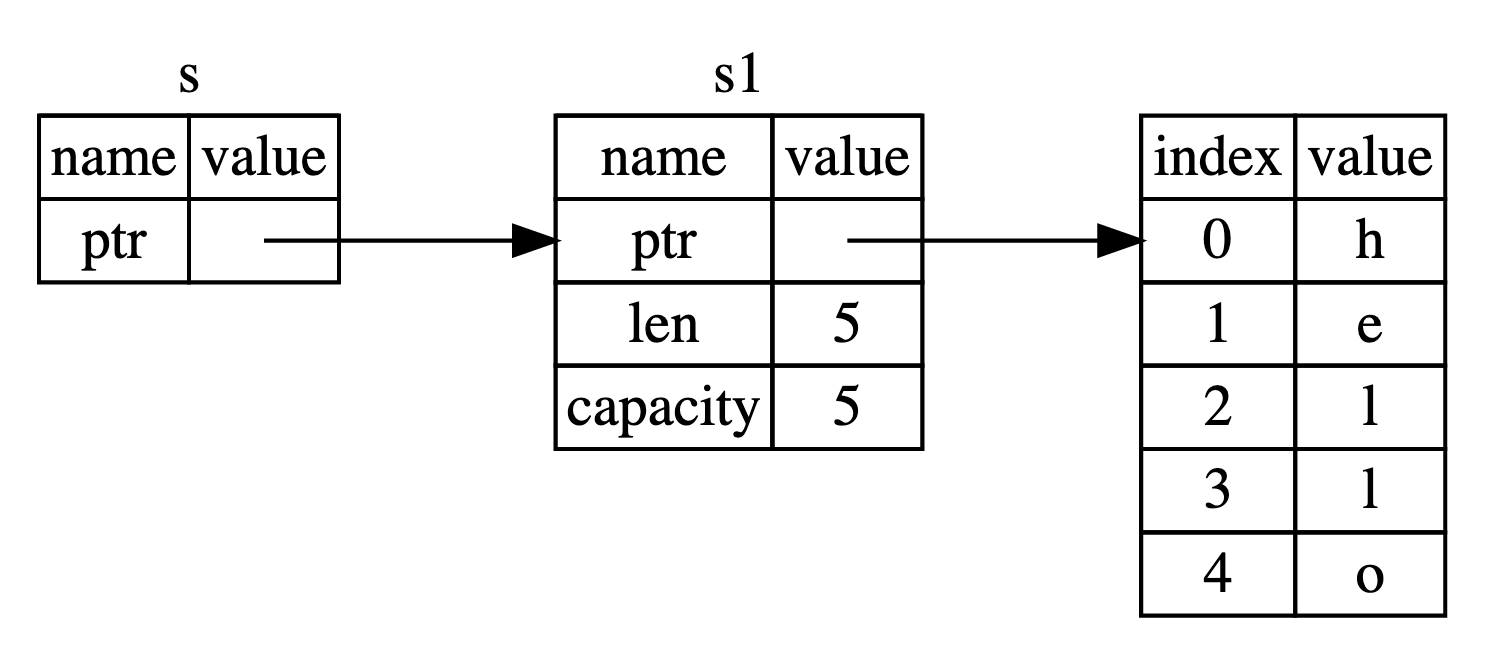
\includegraphics[width=0.5\textwidth]{images/string-with-ref.png}
\end{center}

And if you borrow something, it's not yours to do with as you wish -- you cannot assign ownership of it (move it), which makes sense because you can't give someone ownership of something you do not own.

By default, references are immutable: if you borrow something, you cannot change it, even if the underlying data is mutable. Attempting to do so will result in -- you guessed it -- a compile time error, where the compiler tells you that you are trying to change something that's immutable. 

Of course, in real life, you would be much more agreeable to letting people borrow your things if there were strong guarantees that it would (1) always be returned and (2) would be returned in the same condition. That would be nice! But until such time as that magical technology is invented, no, you can't borrow my car. Sorry.

Mutable references do exist, but they have to be declared explicitly as such by tagging them as \texttt{\&mut}:

\begin{lstlisting}
fn main() {
    let s1 = String::from("hello");
    let len = calculate_length(&mut s1);
    println!("The length of '{}' is {}.", s1, len);
}

fn calculate_length(s: &mut String) -> usize {
    s.len()
}
\end{lstlisting}

Mutable references come with  some big restrictions: (1) while a mutable reference exists, the owner can't change the data, and (2) there can be only one mutable reference at a time, and when there is, there can be no immutable references. This is, once again, to prevent the possibility of a race condition. These two restrictions ensure that there aren't concurrent accesses to the data when writes are possible. There's also a potential performance increase where values can be cached (including in CPU registers; we'll come to that later) without worry that they will get out of date.

As long as there are no mutable references, there can be arbitrarily many immutable references at the same time, because reads don't interfere with reads and a race condition does not occur if there are only reads. 

References cannot outlive their underlying objects. Below is an example from the official docs that will be rejected by the borrow checker, because the reference returned in \texttt{dangle} refers to memory whose owner \texttt{s} goes out of scope at the end of the function:

\begin{lstlisting}[language=Rust]
fn main() {
    let reference_to_nothing = dangle();
}

fn dangle() -> &String {
    let s = String::from("hello");
    &s
}
\end{lstlisting} 

In C this would be a ``dangling pointer'' (a pointer that's pointing to a location that is no longer valid). I see this kind of error a lot in C programs where someone has stack allocated a structure and then wants to pass it to another thread and does so with the address-of operator. It compiles and might even work sometimes at runtime, but is still wrong and can eventually lead to a bug that bites you. 

If we actually try to compile the previous code example, the compiler says something about giving the value a lifetime. We'll come back to the idea of lifetimes soon.

\paragraph{Non-Lexical Lifetimes.} A more recent improvement to Rust's borrow checking is called non-Lexical lifetimes. Consider the small block of code below:
\begin{lstlisting}[language=Rust]
fn main() {
    let mut x = 5;

    let y = &x;
    println!("{}", y);

    let z = &mut x;
}
\end{lstlisting}

Under the old rules, the compiler would not allow creation of the mutable reference \texttt{z} because \texttt{y} has not gone out of scope. It would consider \texttt{y} to be valid until the end of the function. The improvement of NLL is that the compiler can see that \texttt{y} is no longer used after the \texttt{println!} macro and the \texttt{z} reference is okay to create. The compiler will then make it so that \texttt{y} is removed as soon as it's no longer needed so the \texttt{z} reference will not exist at the same time and all is fine.

\subsection*{Slices}
The \textit{slice} concept exists in a few other programming languages, and if you have experience with them this will certainly help. A slice is a reference (yes, a reference in the sense of the previous section) to a contiguous subset of the elements of a collection. This is what you do if you need a part of an array (the typical example for that being a substring of an existing string). If our code looks like this:

\begin{lstlisting}[language=Rust]
fn main() {
    let s = String::from("hello world");
    let hello = &s[0..5];
    let world = &s[6..11];
}
\end{lstlisting}

The representation of the slice looks like~\cite{rustdocs}:
\begin{center}
	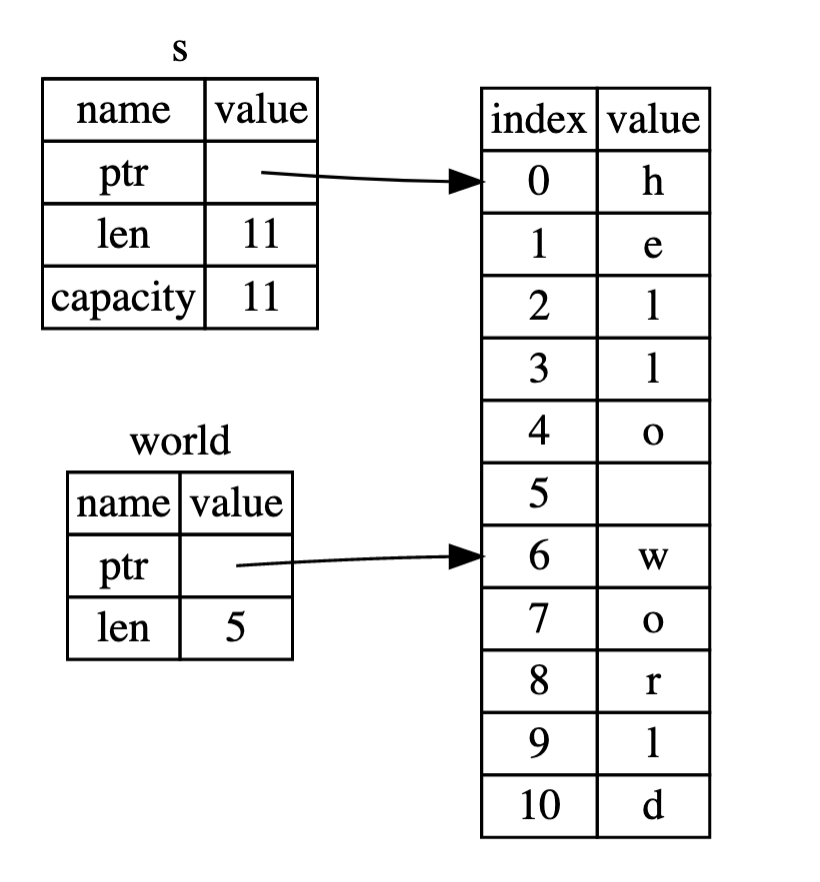
\includegraphics[width=0.3\textwidth]{images/string-slice.png}
\end{center}

Slices can also apply to vectors and other collections; not just strings. As with the other kinds of references we've learned about, the existence of a slice prevents modification of the underlying data. Just as with references, slices prevent race conditions on collections but also avoid (as much as possible) the need to copy data (slow).

\subsection*{Unwrap the Panic}
A quick digression: a lot of functions we use return \texttt{Result} types. These return either \texttt{Ok} with the type we expected, or \texttt{Err} with an error description. To get the type you want, you need to unpack the result.

If we try to open a file but the file doesn't exist, that's an error but one that's foreseeable and we can handle it. There's three ways to handle it: a \texttt{match} expression (this is like the \texttt{switch} statement), \texttt{unwrap()}, and \texttt{expect()}. 

You may be tempted to jus always use \texttt{unwrap()} because it gives you the result and calls the \texttt{panic!} macro if there's an error. This, however, just shows you the lower level error that is the problem and you are denying yourself the opportunity to add information that will help you debug. For that reason, it's better to use \texttt{expect()}, which lets you add your own error message that will make it easier to find out where exactly things went wrong.

It's recommended to use \texttt{Result} types for functions you write too. Make your future self happy by giving yourself the information you need to debug what's gone wrong!

\section*{Fearless Concurrency}
More than just trying to prevent memory problems by making them compiler errors, Rust is also intended to make concurrency errors compile-time problems too! That's actually difficult, of course, but the good news is that the ideas of ownership and borrowing and such are at the heart of how concurrency problems are avoided.

Let's actually take a minute to talk about concurrency and how it helps. The basic idea is that by making our program concurrent, we can get work done faster or accomplish more work in the same amount of time. We'll be revisiting the details of this later and considering the limits of it, but for now you can just imagine it is a good thing at least some of the time.

The problem with concurrency is that it brings new problems with it: race conditions, deadlock, that sort of thing. Making your program faster is great, but not if it's at the cost of the answers being incorrect (or your program failing to produce an answer some of the time).

If the compiler can help with making sure your concurrent program is correct, it doesn't make your program faster directly, but it helps indirectly. If you can be (more) sure of the correctness of your code, you don't have to spend as much time testing it before you can deploy it and move on to the next thing. Also, if the bug is prevented from being introduced in the first place, you don't have to spend time debugging it and fixing it, which lets you spend more time on speeding up other things. And honestly, if you are looking at a piece of code that is super business critical, anything that adds to your confidence that no issue has been introduced makes it that much easier to make that change you want to make.

\paragraph{Threads.} Rust uses threads for concurrency, with a model that resembles the create/join semantics of the POSIX pthread. If you are unfamiliar with pthreads, the course repository has a PDF refresher of the topic. We will talk about the Rust way, but the background material will help you to be caught up.

So you want to create a thread! The mechanism for doing so is referred to as spawning a thread. Here's a quick example from the official docs~\cite{rustdocs}:

\begin{lstlisting}[language=Rust]
use std::thread;
use std::time::Duration;

fn main() {
    let handle = thread::spawn(|| {
        for i in 1..10 {
            println!("hi number {} from the spawned thread!", i);
            thread::sleep(Duration::from_millis(1));
        }
    });

    for i in 1..5 {
        println!("hi number {} from the main thread!", i);
        thread::sleep(Duration::from_millis(1));
    }

    handle.join().unwrap();
}
\end{lstlisting}

A few things make this significantly different from the pthread model that we are used to. First of all, the thread being created takes as its argument a \textit{closure} -- this is an anonymous function that can capture some bits of its environment. The spawn call creates a \texttt{JoinHandle} type and that's what we use to call \texttt{join}, which is to say, wait for that thread to be finished. As we expect from pthreads, if calling join on a thread that is not finished, the caller waits until the thread is finished.

This is a simple example that works, but fails to capture the complexity of actually working with threads, because there's no data being moved between threads. That sometimes happens, but you can't count on it. There are three ways that we can get data from one thread to another: capturing, message passing, and shared state.

\paragraph{Capturing.} 
Capturing calls back to the earlier mention that a closure captures some of its environment. That is, the body of the function can reference variables that were declared outside of that function and in the context where \texttt{thread::spawn} was called. The compiler will analyze the request and try to figure out what needs to happen to make it work, such as borrowing the value, as in this example (also from the docs):

\begin{lstlisting}[language=Rust]
use std::thread;

fn main() {
    let v = vec![1, 2, 3];

    let handle = thread::spawn(|| {
        println!("Here's a vector: {:?}", v);
    });

    handle.join().unwrap();
}
\end{lstlisting}

The only problem is: this example does not work. The compiler is not sure how long the thread is going to live and therefore there's a risk that a reference to \texttt{v} held by the thread outlives the actual vector \texttt{v} in the main function. How do we fix that?

Well, I had the idea that if I put something after the \texttt{join()} call that uses \texttt{v}, then the compiler should know that \texttt{v} has to remain in existence until after the thread in question. Yet, it still reports the error E0373 that says the thread might outlive the borrowed value. This actually got me thinking about why this didn't work and I decided to ask some of the compiler devs. It has to do with the fact that a thread isn't really a first-class construct in Rust, and the ``lifetime'' of arguments that you pass has to be sufficiently long. We'll learn about lifetimes soon.

Anyway, the error message suggests what you actually want in this scenario: to move the variables into the thread. To do so, specify \texttt{move} before the closure: \texttt{let handle = thread::spawn(move || \{}... That results in the transfer of ownership to the thread being created. You can also copy if you need.

\paragraph{Message Passing.} Sometimes threads want to communicate in a way that isn't one-way communication at the time that the thread is being created. For that, a possibility is message-passing. This mechanism of communication may seem familiar from previous experience with various UNIX mechanisms like pipes and message queues. This strategy is very structured and generally safer than shared memory. 

The ownership mechanic of message passing is like that of postal mail. When you write a physical letter and mail it to someone, you relinquish your ownership of the letter when it goes in the mailbox, and when it is delivered to the recipient, the recipient takes ownership of that letter and can then do with it as they wish.

So you want to have two threads communicate: the Rust metaphor for this is called a \textit{channel}. It has a transmit end (where messages are submitted) and a receive end (where messages arrive). The standard model is multiple-producer, single-consumer; that is, lots of threads can send data via the sending end, but in the end it all gets delivered to one place. Think of that like postal mail as well; I can drop a letter to you in any postbox or post office, but they will all be delivered to your mailbox where you collect them in the end.

Okay, enough talk, let's make one~\cite{rustdocs}:
\begin{lstlisting}[language=Rust]
use std::sync::mpsc;
use std::thread;

fn main() {
    let (tx, rx) = mpsc::channel();

    thread::spawn(move || {
        let val = String::from("hi");
        tx.send(val).unwrap();
    });

    let received = rx.recv().unwrap();
    println!("Got: {}", received);
}
\end{lstlisting}

The channel constructor returns a tuple with the transmitting end \texttt{tx} and receiving end \texttt{rx}. We'll then send the transmitting end into the thread and have it send a message to the main thread. The main thread will wait until the message is there and then get it. This does mean that \texttt{recv()} is blocking and there is a corresponding \texttt{try\_recv()} which is nonblocking. You may have already covered nonblocking I/O in a previous course; if not we will return to that subject soon.

If you want to have multiple transmitting ends, you need only use \texttt{clone} on the transmitter and hand those out as needed. 

As a small technical note, the type you want to send via a channel has to implement the \texttt{Send} trait (think of traits like interfaces). Almost all basic types in Rust have this trait, and any programmer-defined type that is composed entirely of types that have it will also have that trait.  

\paragraph{Mutex and Reference Counting}
If you don't want to use message passing for some reason (and performance is a reason, if it's borne out by your testing/data) then there is fortunately the ability to use a mutex for mutual exclusion. We know how these work, so let's skip the part where I make some analogy about them. 

What's different about the mutex in Rust is that the Mutex wraps a particular type. So it is defined as \texttt{Mutex<T>} and if you want an integer counter, you create it as \texttt{Mutex::new(0);}. This way, the mutex goes with the value it is protecting, making it much more obvious what mutex goes with what data, and making it so you have to have the mutex to access the data. And sample from the docs\cite{rustdocs}:

\begin{lstlisting}[language=Rust]
use std::sync::Mutex;

fn main() {
    let m = Mutex::new(5);

    {
        let mut num = m.lock().unwrap();
        *num = 6;
    }

    println!("m = {:?}", m);
}
\end{lstlisting}

In addition to forcing you to acquire the mutex before you can make any use of the internal value, the lock is automatically released when the \texttt{num} variable goes out of scope; the type of \texttt{num} is a \texttt{MutexGuard} which is our ``possession'' of the lock; when that possession ends, the mutex is automatically unlocked. This means you want, generally, to use the manual-scoping \texttt{ \{ } and \texttt{ \} } braces to ensure that the lock is released when you're done with it and not just at the end of the function or loop.

The use of the mutex in the above program is obviously unnecessary, since there's only the one thread. If we want to use it in multiple threads, we need multiple threads to access it. But we can't, unfortunately, just say that references will do! The mutex type has to outlive the other threads and such and the compiler will suggest moving it... But we can't move it into more than one thread, because that violates our rule about having only one owner. What now?

It looks like we have to break a rule: we need the ability to share ownership of some memory. 

\paragraph{Smart Pointers and Reference Counting}
This takes us down a slight digression, to the subject of smart pointers and reference counting. We know what pointers are from C and \CPP, and if you have sufficient experience with \CPP you will know that smart pointers exist in that language too! We'll talk about two kinds of smart pointer right now, the Box and the Reference-Counting type.

The \texttt{Box<T>}is an easy way to put some data on the heap rather than the stack. This is good for a situation where you, for example, take input from a user and you don't know in advance how big it's going to be, or when you have some data that you want to transfer ownership of rather than copy (for performance reasons, obviously). You create a Box with \texttt{Box::new(...)} as expected, and it's heap allocated with all the usual things that come with it in rust, like ownership and that it gets dropped if the owner goes out of scope.

The reference counted smart pointer, however, is the thing that allows for shared ownership. There are some reasons why we might want this, even in a single-threaded program, such as a graph data structure. But the main idea is that you can share ownership as much as you like, and the value only goes away when the last reference to it is dropped (reference count goes to zero). 

To make a reference-counted object, it's of type \texttt{Rc<T>}and that creates the type; if you want to make another reference, use \texttt{clone()} and that increases the reference count. When references are dropped, the count decreases.

It is important to note that reference types can leak memory! If you've chosen this route for managing data in your program, there is a possibility of forming a cycle in the reference types. If such a cycle is formed, the memory will never be dropped. This is undesirable, of course.

Right, so we have everything we need now to pass the mutex around, right? Well, almost. \texttt{Rc<T>} won't work when we try to pass it between threads, because the compiler says it cannot be sent between threads safely. This is because the management of its internal counter is not done in a thread-safe way, and if we want that, we need the \textit{atomic} reference counted type, which is \texttt{Arc<T>}. It is perhaps slightly slower than the regular reference counted type, so you won't want to choose it in every scenario, but it's exactly what we need here.

Here's an example of using an atomic reference counted type for setting up a handler for the Ctrl-C (SIGINT); this is modified from a program I wrote that listens for connections and spawns threads if a client connects: 

\begin{lstlisting}[language=Rust]
use std::sync::Arc;
use std::sync::atomic::{AtomicBool, Ordering};

fn main() {
   let quit = Arc::new(Mutex::new(false));
    let handler_quit = Arc::clone(&quit);
    ctrlc::set_handler(move|| {
        let mut b = handler_quit.lock().unwrap();
        *b = true;
    }).expect("Error setting Ctrl-C handler");
 
    while !(*quit.lock().unwrap()) {
    	// Do things
    }
}
\end{lstlisting}

In this example, I use a mutex to protect a boolean that's used concurrently (even if it's not in two threads): once in main and once in the handler. 

We should also still remember that there exists the possibility of a deadlock in Rust, even if the mutex is automatically unlocked for us. Nothing prevents thread 1 from acquiring mutex A then B and thread 2 from concurrently acquiring B then A. The language cannot solve all concurrency problems, unfortunately.

We just learned how to break a rule (single ownership) and... we liked it. Maybe we can break some more? Maybe we \textit{have} to break some more?

\bibliographystyle{alphaurl}
\bibliography{459}


\end{document}